\documentclass[a4paper,10pt]{report}
\usepackage[top=2cm, bottom=2cm, left=2cm, right=2cm]{geometry}
\usepackage[utf8x]{inputenc}
\usepackage[T1]{fontenc}
\usepackage[french]{babel} 
\usepackage{lmodern} % Pour changer le pack de police
\usepackage{makeidx}
\usepackage{hyperref}
\usepackage{uml}
\usepackage{graphicx}
\usepackage{listings}
\title{Projet tutoré de C++}
\author{\textsc{Jorandon} Guillaume et \textsc{Simon} Clément\\\normalsize{IUT d'Amiens}\\\normalsize{Tuteur : Laurent \textsc{Delahoche}}}
\date{6 juillet 2016}

\definecolor{mygreen}{rgb}{0,0.6,0}
\definecolor{mygray}{rgb}{0.5,0.5,0.5}
\definecolor{mymauve}{rgb}{0.58,0,0.82}

\lstset{ %
  backgroundcolor=\color{white},   % choose the background color; you must add \usepackage{color} or \usepackage{xcolor}
  basicstyle=\footnotesize,        % the size of the fonts that are used for the code
  breakatwhitespace=false,         % sets if automatic breaks should only happen at whitespace
  breaklines=true,                 % sets automatic line breaking
  captionpos=b,                    % sets the caption-position to bottom
  %commentstyle=\color{mygreen},    % comment style
  deletekeywords={...},            % if you want to delete keywords from the given language
  escapeinside={\%*}{*)},          % if you want to add LaTeX within your code
  extendedchars=true,              % lets you use non-ASCII characters; for 8-bits encodings only, does not work with UTF-8
  frame=single,	                   % adds a frame around the code
  keepspaces=true,                 % keeps spaces in text, useful for keeping indentation of code (possibly needs columns=flexible)
  %keywordstyle=\color{blue},       % keyword style
  keywordstyle=\bfseries\color{green!40!black},
  commentstyle=\itshape\color{purple!40!black},
  identifierstyle=\color{blue},
  stringstyle=\color{orange},
  otherkeywords={*,...},           % if you want to add more keywords to the set
  numbers=left,                    % where to put the line-numbers; possible values are (none, left, right)
  numbersep=5pt,                   % how far the line-numbers are from the code
  numberstyle=\tiny\color{mygray}, % the style that is used for the line-numbers
  rulecolor=\color{black},         % if not set, the frame-color may be changed on line-breaks within not-black text (e.g. comments (green here))
  showspaces=false,                % show spaces everywhere adding particular underscores; it overrides 'showstringspaces'
  showstringspaces=false,          % underline spaces within strings only
  showtabs=false,                  % show tabs within strings adding particular underscores
  stepnumber=1,                    % the step between two line-numbers. If it's 1, each line will be numbered
  stringstyle=\color{mymauve},     % string literal style
  tabsize=2,	                   % sets default tabsize to 4 spaces
}

\makeindex
\begin{document}

\maketitle

\tableofcontents

\chapter*{Introduction}
\addcontentsline{toc}{chapter}{Introduction}
Dans le cadre du DUT Informatique AS de l'IUT d'Amiens, nous avons été amenés à mettre en pratique ce que nous avions étudié tout au long de l'année dans un projet tutoré de développement applicatif en C++. Le sujet était imposé et demandait la réalisation d'un \textit{fork} de Bomberman, un \textit{puzzle game} apparu en 1983 sur \textit{ZX Spectrum}, puis popularisé notamment sur les consoles de la firme \textit{Nintendo}. Ce jeu-vidéo très simple dans son principe met en scène un personnage dans un décor fermé, qui a la capacité de poser des bombes afin de progresser dans le jeu. C'est un exemple parfait pour mettre en pratique les notions de programmation et d'algorithmique apprises en cours, puisqu'il implique la création d'un moteur de jeu simple.

Nous allons dans ce rapport revenir sur les différentes étapes de la conception et de la réalisation de notre Bomberman. Nous reviendrons d'abord sur la pré-conception du projet : interprétation du sujet, choix des technologies. Puis nous expliciterons dans une deuxième partie les détails de la réalisation : analyse descendante, diagrammes de classe, boucle de jeu, etc.

Le code est téléchargeable en clonant le dépôt du projet. Pour compiler le projet, exécutez le makefile (attention à bien avoir correctement installé SFML au bon endroit). Exemple sous GNU/Linux :
\lstinputlisting[language=bash]{install.sh}

\chapter{Génèse}
\section{Interprétation du sujet}
La première étape a été d'interpréter le sujet donné. Le minimum exigé par le sujet comporte plusieurs éléments de base.
\begin{description}
 \item[Principe du jeu de base] Le jeu doit correspondre à une version minimaliste de Bomberman. Cela peut sembler évident, mais il faut s'assurer de connaître un minimum le jeu afin de ne pas faire de hors-sujet. Bien heureusement, Bomberman est un jeu extrêmement connu.
 \item[Interface graphique] Le jeu doit être implémenté dans une interface graphique utilisateur, et non pas en ligne de commande.
 \item[Gestion du déplacement] Le personnage doit être capable de se mouvoir, contrôlé par le joueur.
 \item[Gestion des collisions avec le décor] Le personnage ne doit pas traverser les obstacles, ni sortir des limites de la carte.
 \item[Pose de bombes] Le personnage doit être capable de poser une bombe, qui explose au bout d'un court instant en propageant une explosion.
\end{description}

Nous avons cependant très vite décidé de nous fixer plusieurs exigences supplémentaires, afin d'obtenir un jeu plus achevé et jouable.
\begin{description}
 \item[Présence d'un menu] Plutôt que de lancer directement la partie au démarrage du programme, et de fermer celui-ci à la fin de la partie, un menu présente une interface moins austère à l'utilisateur.
 \item[Affichage texturé] Plutôt que de représenter les éléments du jeu par des polygones colorés, l'utilisation de textures (\textit{sprites}) rend le jeu plus élégant, en plus d'apporter des problématiques de programmation supplémentaires.
 \item[Textures animées] Des animations rendent le jeu moins statiques et posent des problèmes de gestion du temps.
 \item[Deux joueurs contrôlés par deux humains] Le jeu devient ainsi réellement jouable, avec un objectif clair : annihiler son adversaire.
 \item[Destruction des éléments du jeu] La bombe peut détruire certains blocs et tuer les joueurs.
\end{description}

Ainsi, un cahier des charges se dégage du sujet initial, ce qui nous donne un certains nombre d'objectifs clairs à remplir.

\section{Choix des technologies}
Le sujet n'imposait que le langage de programmation (C++). Ainsi, l'utilisation de bibliothèques tierces, notamment pour les graphiques, était laissé à la libre appréciation de chaque binôme. Nous avons décidé de ne pas partir sur la bibliothèque graphique présentée en cours (Allegro), pour utiliser plutôt SFML (Simple and Fast Multimedia Library)\footnote{SFML est distribuée selon les termes de la \href{https://opensource.org/licenses/Zlib}{licence zlib/png}.}. Cette API, créée par Laurent \textsc{Gomila}, un développeur français, présente plusieurs avantages. Elle est écrite en C++ et entièrement orientée objet, et est très modulaire. De plus, elle est portable, ce qui signifie qu'un programme qui l'utilise peut être compilé et tourner sous Windows, macOS et GNU/Linux sans problème. Enfin, l'un de nous deux utilisait déjà SFML, ce qui permet de gagner du temps sur l'apprentissage de l'API.

Nous avons aussi utilisé doxygen pour commenter le code. Doxygen est un logiciel de génération de documentation qui nous a permis de créer facilement la documentation du code.

\chapter{Développement}
\begin{figure}
 \begin{center}
  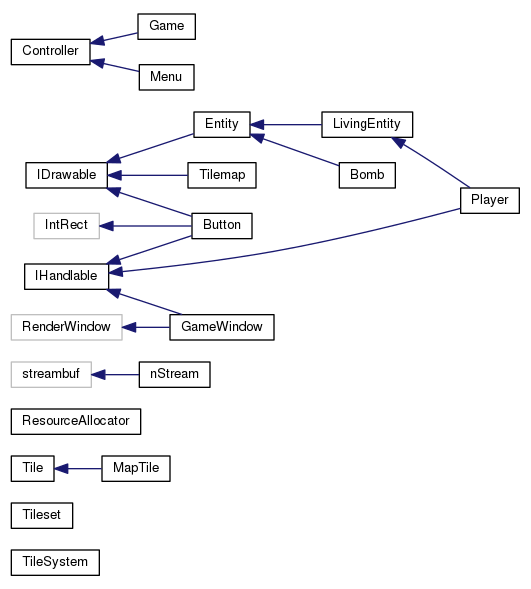
\includegraphics[scale=0.44]{uml.png}
 \end{center}
 \caption{Diagramme de classe du projet}
 \label{uml}
\end{figure}
\section{Analyse descendante}
Avant de commencer à coder, il nous a fallu dégager les fonctionnalités principales du programme et les articulations entres elles. Pour cela, on réalise une analyse descendante de la boucle de jeu. Celle-ci se décompose en plusieurs étapes : récupération des entrées utilisateur, mise à jour du jeu, raffraichissement de l'affichage.
\begin{itemize}
 \item Début du jeu : on charge les ressources, on initialise les positions des joueurs, l'état initial de la carte.
 \item Entrée dans la boucle de jeu : elle dure tant qu'aucun joueur n'a gagné (en tuant l'adversaire).
 \item On récupère le temps écoulé depuis le dernier début de cycle, afin de préparer la mise à jour de l'état du jeu.
 \item On récupère les entrées utilisateur.
 \item On met à jour les éléments du jeu en fonction du temps écoulé (et éventuellement des entrées utilisateur).
 \item On met à jour l'affichage de chaque élément.
 \item Fin de la boucle de jeu (début d'un nouveau cycle ou sortie en cas de victoire).
 \item Fin du jeu : on libère les ressources allouées.
\end{itemize}
Comme on a décidé d'intégrer un menu principal, l'intégralité des étapes ci-dessus s'exécute quand on sélectionne dans le menu l'option Jouer. Ainsi, on peut rejouer une fois la partie terminée, en relançant toutes ces étapes. 

On peut ensuite créer un modèle UML des classes nécessaires. Nous avons décidé très vite d'utiliser une version simplifiée \textit{design pattern} MVC\footnote{Modèle - Vue - Contrôleur}. Cette manière d'organiser le code permet d'avoir une meilleur clarté, et une grande modularité qui rend le code ouvert à des améliorations futures. Cependant, on parle bien ici de modèle simplifié, puisque les vues ici sont des fenêtres, qui sont réduites à leur rôle de contexte d'affichage.

Le détail des classes (diagrammes de classe, graphes d'héritage et de collaboration) est disponible dans le document refman.pdf, généré par doxygen, mais la figure \ref{uml} décrit plus succintement les relations d'héritage entre les classes.

\section{Un point sur le Tile mapping}
Dans un jeu vidéo 2D de type Bomberman ou Mario, les joueurs évoluent dans un monde défini sous forme de grille : chaque case de la grille contient un élément de décor, qui possède des propriétés. C'est bien plus pratique que de définir le monde comme une grande image, car celle-ci contient nécessairement beaucoup d'élements qui se répètent. Il est donc plus aisé de créer chacun de ses éléments (des tuiles, ou \textit{tiles}) à partir d'une base (un \textit{sprite sheet}), et de les afficher x fois quand c'est nécessaire. Ce type de level design s'appelle le \textit{Tile mapping}, et il a permis à l'époque où la place en mémoire d'une machine était une chose rare de réaliser des jeux visuellement riches et aux niveaux complexes et construits. C'est cette méthode qui a été retenue pour le projet, car elle est non seulement adaptée au jeu demandé, mais en plus assez facile à mettre en place. D'autant plus que des \textit{sprite sheets} de jeux célèbres sont accessibles gratuitement sur le web (figures \ref{rawSheet} et \ref{customSheet}).

Sur nos \textit{sprite sheets} utilisés dans le projet, les tuiles sont collées les unes à la suite des autres, mais on peut voir sur le \textit{sprite sheet} de Super Bomberman 4 qu'un espace de 1 pixel existe pour mieux distinguer les tuiles. Ceci ne change rien au principe de base.

\begin{figure}
 \begin{center}
  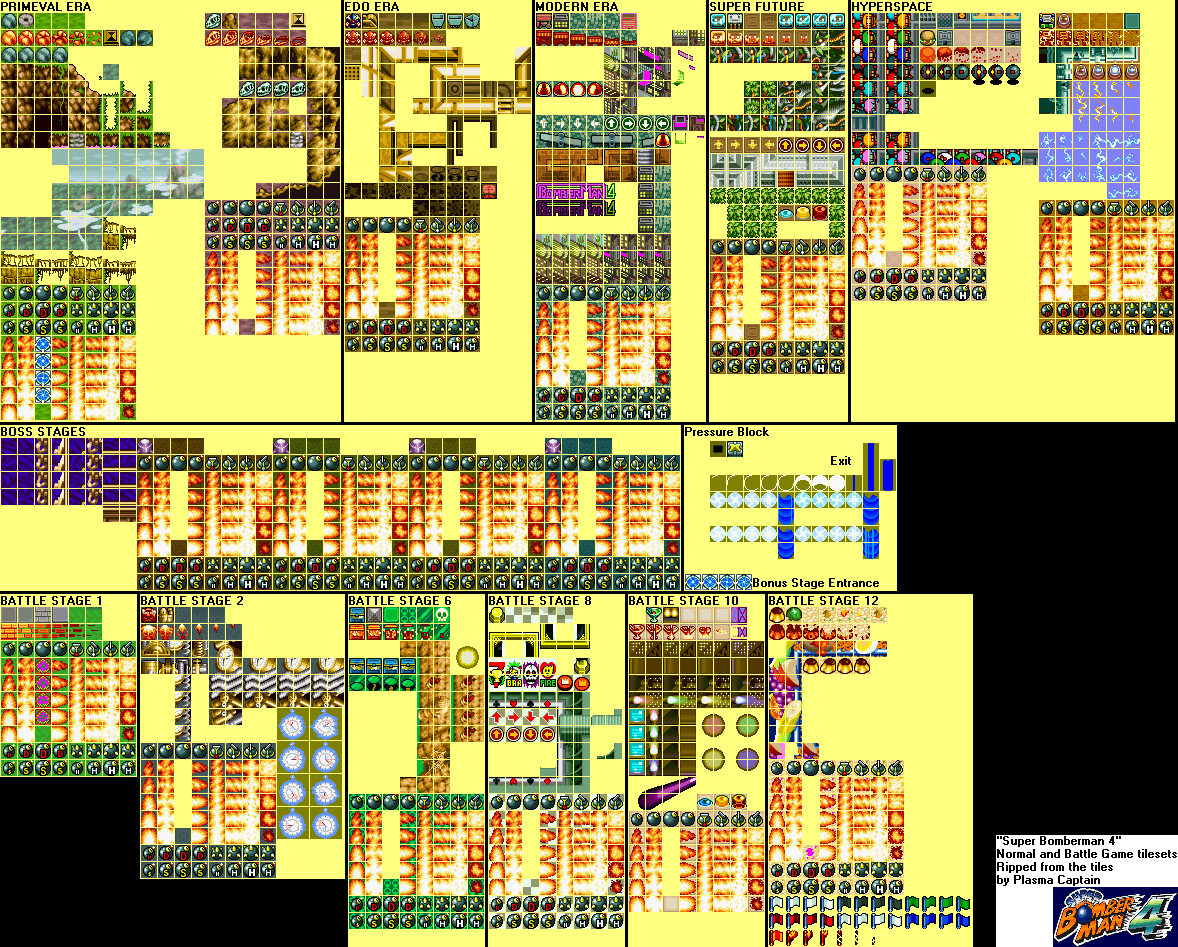
\includegraphics[scale=0.4]{rawSheet.png}
 \end{center}
 \caption{\textit{Sprite sheet} de Super Bomberman 4 trouvé sur \href{http://www.spriters-resource.com/fullview/60516/}{spriters-resource.com}}
 \label{rawSheet}
\end{figure}
\begin{figure}
 \begin{center}
  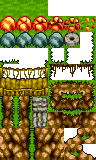
\includegraphics[scale=0.44]{customSheet.png}
 \end{center}
 \caption{\textit{Sprite sheet} modifié pour le projet}
 \label{customSheet}
\end{figure}

\section{Description des classes}
Le projet a été découpé de manière logique en classes. Chaque classe va être ici brièvement résumé, mais le détail des attributs et méthodes de chaque classe est donné dans le refman.pdf généré par doxygen.
\subsection{Interfaces}
Une interface est une notion qui n'est pas formalisée en C++ : il s'agit d'un ensemble de méthodes abstraites et d'attributs qu'une classe qui implémente l'interface possèdera automatiquement : la description des méthodes n'est pas faite dans l'interface, mais dans la classe qui l'implémente. Ici, on a utilisé ce principe pour que des classes très différentes puissent implémenter une caractéristique commune.
\subsubsection{\texttt{IDrawable}}
\lstinputlisting[language=C++, firstline=100, lastline=110]{classes.cpp}
Les \texttt{IDrawable} sont des éléments qui peuvent être affichés par le moteur de jeu : à ce titre, ils contiennent un \texttt{TileSystem} et une méthode abstraite \texttt{void draw(GameWindow *window)}, que les classes qui implémentent \texttt{IDrawable} devront implémenter pour définir la manière dont l'élément est affiché.
\subsubsection{\texttt{IHandlable}}
\lstinputlisting[language=C++, firstline=134, lastline=139]{classes.cpp}
Les \texttt{IHandlable} sont des éléments qui peuvent être contrôlés d'une manière ou d'une autre par un utilisateur : dit autrement, un élément qui implémente cette interface possède des évènements internes. L'interface ne comporte qu'une méthode abstraite, \texttt{void manageEvents(sf::event \&event, void *args=NULL)}, qui prend en paramètre l'évènement à analyser et un pointeur générique sur un ou plusieurs arguments potentiels.
\subsection{Modèles}
Les modèles sont les classes qui contiennent des données : dans notre cas, ils décrivent les éléments du moteur de jeu comme le joueur, la carte, une bombe ou un bouton. Attention cependant, tous les modèles ne sont pas des éléments affichables (rappel : un élément affichable hérite de \texttt{IDrawable}).
\subsubsection{\texttt{Tileset}}
\lstinputlisting[language=C++, firstline=274, lastline=308]{classes.cpp}
Un \texttt{Tileset} contient les informations brutes de découpage d'un \textit{sprite sheet} : il possède une hauteur de tuile et une largeur de tuile, un nombre de lignes et de colonnes, mais surtout une texture. Un \texttt{Tileset} contient aussi les méthodes qui permettent de créer des \texttt{Tile} par découpage.
\subsubsection{\texttt{Tile}}
\lstinputlisting[language=C++, firstline=225, lastline=243]{classes.cpp}
Un \texttt{Tile} est le découpage d'un Tileset en un ou plusieurs \textit{sprites} : bien que la plupart des \textit{Tile} ne possèdent qu'un \textit{sprite}, certains en possèdent plusieurs, par exemple car ils sont animés, ou car il possèdent plusieurs états possibles (selon l'état de l'entité qui l'exploite par exemple). En tant que tel, un \texttt{Tile} n'est pas directement utilisable, il doit être encapsulé dans une classe qui les répertorie et les indexe (c.f plus bas).
\subsubsection{\texttt{MapTile}}
\lstinputlisting[language=C++, firstline=157, lastline=172]{classes.cpp}
Un \texttt{MapTile} est un type de \texttt{Tile} un peu particulier, qui stocke des informations supplémentaires destinées aux cartes : ces informations permettent de savoir si la Tuile peut être détruite, ou si elle est collisionnable (de l'herbe est indestructible et non collisionnable, à l'inverse d'une brique par exemple).
\subsubsection{\texttt{TileSystem}}
\lstinputlisting[language=C++, firstline=310, lastline=337]{classes.cpp}
Un \texttt{TileSystem} indexe des \texttt{Tile} provenant d'un même \texttt{Tileset} : cette classe encapsule tout les éléments de \textit{tile mapping} précédemment décrits.
\subsubsection{\texttt{Entity}}
\lstinputlisting[language=C++, firstline=112, lastline=132]{classes.cpp}
Une entité est un \textit{asset} quelconque du moteur du jeu, qui évolue sur la carte. Il possède un certain nombre de points de vie, une boîte de collision (le code est prévu pour pouvoir créer aisément plusieurs boîtes de collision si les classes filles en ont besoin), une position, et une horloge interne qui permet de mettre à jour son état. Cette classe est abstraite car elle contient une méthode pure virtuelle, à savoir \texttt{void updateState(Controller *controller, sf::Time \&elapsed, Tilemap *world)}, que les classes filles implémentent pour définir la manière dont l'entité se met à jour en fonction du temps écoulé, de l'état du contrôleur parent et du monde dans lequel évolue l'entité. C'est dans cette méthode que pourront être gérées les collisions.
\subsubsection{\texttt{LivingEntity}}
\lstinputlisting[language=C++, firstline=141, lastline=155]{classes.cpp}
Une entité vivante, à la différence d'une entité, a un caractère mobile. Elle peut être autonome ou contrôlée par un joueur, et possède une orientation et une vitesse.
\subsubsection{\texttt{Player}}
\lstinputlisting[language=C++, firstline=192, lastline=212]{classes.cpp}
Un joueur est une entité vivante contrôlée par le joueur (elle implémente donc \texttt{IHandlable}). Il possède un inventaire de bombes, ainsi que les informations nécessaires pour créer une bombe : apparence, rayon d'explosion. Il possède aussi la capacité de poser une bombe, et perd de la vie de manière graduelle, à chaque fois qu'il est touché (dans le cadre du jeu de base codé, il ne possède qu'un point de vie, mais le code est conçu de telle manière qu'on peut aisément modifier ce facteur).
\subsubsection{\texttt{Bomb}}
\lstinputlisting[language=C++, firstline=1, lastline=16]{classes.cpp}
Une bombe est une entité spéciale qui a une durée de vie limitée, et qui cause des dégats quand elle explose.
\subsubsection{\texttt{Tilemap}}
\lstinputlisting[language=C++, firstline=245, lastline=272]{classes.cpp}
Un Tilemap est un élément affichable qui constitue le plateau de jeu : il stocke une matrice d'indices de \texttt{MapTile}, mais aussi une matrice de métadonnées : en effet, certains \texttt{MapTile} ont des états qui peuvent différer en fonction du temps, et il faut donc stocker ces états sous la forme d'une métadonnée.
\subsubsection{\texttt{Button}}
\lstinputlisting[language=C++, firstline=18, lastline=33]{classes.cpp}
Un bouton est un élément affichable et contrôlable de forme rectangulaire qui déclenche une action quand l'utilisateur clique dessus. Cette classe hérite de \texttt{sf::IntRect}, une classe de SFML qui possède déjà des attributs et des méthodes pour manipuler des objets rectangulaires. Concernant le \textit{callback} (fonction appelée lorsque le bouton est activé), on utilise un pointeur sur fonction qui prend en paramètre un pointeur générique.

\subsection{Vues}
\subsubsection{\texttt{GameWindow}}
\lstinputlisting[language=C++, firstline=80, lastline=98]{classes.cpp}
L'unique vue du jeu se contente de stocker des informations de base sur la taille de la fenêtre en termes de tuiles. Elle intègre aussi une fonction qui permet de rectifier le ratio quand la fenêtre est redimensionnée, mais un bogue de raffraichissement fait que cette méthode n'est pas exploitée, et que la fenêtre a une taille fixe.

\subsection{Contrôleurs}
\subsubsection{\texttt{Controller}}
\lstinputlisting[language=C++, firstline=35, lastline=53]{classes.cpp}
La classe abstraite \texttt{Controller} définit les caractéristiques communes de tout contrôleur : un contexte d'affichage, et diverses listes indexées de ressources. De plus, elle définit plusieurs méthodes virtuelles pour le fonctionnement et la mise à jour du contrôleur. \texttt{void manageEvents()} s'occupe de récupérer tous les évènements de la boucle de jeu. \texttt{void start()} permet de démarrer le contrôleur et contient la boucle de jeu. \texttt{void notifyUpdate()} permet de raffraichir des entités gérées par le contrôleur à des moments précis, quand une entité l'appelle.
\subsubsection{\texttt{Game}}
\lstinputlisting[language=C++, firstline=55, lastline=78]{classes.cpp}
Le contrôleur de jeu stocke les données des joueurs, de la carte, ainsi que des entités non joueur présentes dessus (dans notre jeu, seules les bombes sont implémentées, mais ce fonctionnement nous permettrait d'ajouter aisément \textit{mobs}, \textit{power-ups} et autres entités de jeu). L'évolution de ce contrôleur est fortement soumise au temps, c'est pourquoi il possède un \textit{timer} qui permet de surveiller le temps écoulé entre chaque itération de la boucle de jeu.
\subsubsection{\texttt{Menu}}
\lstinputlisting[language=C++, firstline=174, lastline=190]{classes.cpp}
Le contrôleur de menu stocke juste les boutons et les \textit{sprites} de décoration (ici nul besoin d'encapsuler les \texttt{sf::Sprite} dans des classes, car ils sont directement affichés à l'écran sans aucune information supplémentaire). Ce contrôleur crée à la volée une instance de jeu quand on clique sur le bouton de jeu. Cette organisation permet de ne charger en mémoire les ressources de jeu que quand c'est nécessaire.

\subsection{Divers}
\subsubsection{\texttt{nStream}}
\lstinputlisting[language=C++, firstline=343, lastline=348]{classes.cpp}
Cette structure très simple hérite de \texttt{std::streambuf}, et se comporte comme un \textit{buffer} nul. Son rôle est analogue à celui de \textit{/dev/null} dans les systèmes Unix, et permet de supprimer éventuellement l'affichage de la sortie standard (son rôle prend sens dans la fonction \texttt{main}).
\subsubsection{\texttt{TileType}}
\lstinputlisting[language=C++, firstline=339, lastline=339]{classes.cpp}
Cette énumération permet de définir les types de tuile. 4 sont définis, mais tous ne sont pas utilisés dans notre résultat. \texttt{DEFAULT} décrit une tuile standard. \texttt{RANDOMIZED} décrit une tuile dont la métadonnée dans la carte correspond à son sprite d'affichage. Les métadonnées de ce type de tuile étant initialisées de manière aléatoire, il permet très concrètement de définir une tuile dont l'affichage est aléatoire (exemple : l'herbe dispose de plusieurs variantes de son sprite, ce qui permet à l'affichage de casser l'effet de grille induit par le \textit{tile mapping}).
\subsubsection{\texttt{Orientation}}
\lstinputlisting[language=C++, firstline=341, lastline=341]{classes.cpp}
Cette énumération permet de lister les différentes orientations que peut prendre une entité vivante.
\subsubsection{\texttt{ResourceAllocator}}
\lstinputlisting[language=C++, firstline=214, lastline=223]{classes.cpp}
Cette classe entièrement statique rassemble quelques fonctions utilitaires qui permettent de remplir une liste de ressources indexée.

\section{Détails}
Il y a dans le code plusieurs points de détail qui méritent un éclaircissement. Ces détails correspondent notamment à des notions peu ou pas étudiées en cours, et dont l'utilisation dans ce projet doit être justifiée ou expliquée.
\subsection{La fonction \texttt{main}}
\lstinputlisting[language=C++, firstline=1, lastline=65]{details.cpp}
La fonction \texttt{main} a ici plusieurs rôles : lire et traiter les éventuels arguments de la ligne de commande, et lancer le contrôleur principal. Détaillons la bloc par bloc.
\subsubsection{Déclaration des variables}
On a un tampon nul, un pointeur sur le contrôleur principal, une fenêtre de jeu, un pointeur sur le \textit{buffer} de la sortie standard, une variable pour lire les options de la ligne de commande, et un autre qui stockera la taille de tuile (nécessaire pour créer la fenêtre). L'instruction \texttt{cout.rdbuf(\&nullStream)} retourne le \textit{buffer} par défaut de la sortie standard, tout en le remplaçant par notre tampon nul. Ainsi, les affichages de déboguage sont masqués par défaut.
\subsubsection{Cas du mode de déboguage}
Il est cependant possible de rétablir cet affichage de plusieurs manières. le premier est le mode de déboguage, un flag défini à la compilation qui permet de forcer l'affichage des informations sur la sortie standard, en rétablissant le tampon par défaut. 
\subsubsection{Traitement des entrées de la ligne de commande}
Le programme peut admettre plusieurs arguments en entrée : 
\begin{description}
 \item[-h] affiche l'aide et quitte le programme ;
 \item[-v] \textit{verbose mode}, qui rétablit l'affichage de la sortie standard ;
 \item[-s SIZE] modifie la taille par défaut d'une tuile. 
\end{description}
\subsubsection{Instanciation du contrôleur principal}
Une fois les options de la ligne de commande lus, on crée la fenêtre avec la bonne taille. Puis on instancie le contrôleur principal, et on le lance. la fonction \texttt{mainController->start()} ne se termine que quand l'utilisateur ferme la fenêtre ou quitte le jeu.
\subsubsection{Fermeture du programme}
Il ne reste alors plus qu'à désallouer le contrôleur principal et rétablir le tampon de la sortie standard (ne pas le faire peut entraîner un crash de l'application).
\subsection{De l'utilisation de la classe \texttt{std::vector}}
À la fin de la conception, au moment de commencer l'implémentation en C++, la question de l'utilisation ou non de \texttt{std::vector} s'est posée. Cette classe de la STL\footnote{\textit{Standard Template Library}, la bibliothèque standard du C++.} est, pour simplifier très grossièrement, une alternative aux tableaux C classiques pour stocker des informations indexées sous forme de tableau, et dont la taille peut évoluer à tout moment. C'est ce qu'on appelle une classe conteneur. Nous avons en effet en plusieurs endroits du code besoin de supprimer un élément du tableau, ou de lui ajouter des entrées. Bien que tout ceci soit possible avec un tableau C (c'est d'ailleurs comme cela que fonctionne la classe \texttt{std::vector} en interne), l'utilisation de cette solution nous permet de nous affranchir de la réécriture d'une couche d'abstraction, tout en profitant des fonctionnalités avancées du C++ (comme les itérateurs). Il est vrai que les objectifs du projet tutoré prévoyaient la gestion dynamique de la mémoire et la manipulation de pointeurs : cette composante reste bien présente dans notre projet, et est utilisée à de nombreux endroits (par exemple, la déallocation des entrées des \texttt{std::map}\footnote{\texttt{std::map} est une autre classe conteneur très puissante de la STL, qui permet de stocker des entrées indexées par un indice quelconque (et non plus seulement un entier auto-incrémentiel comme c'est le cas pour un tableau ou un \texttt{std::vector}. Par exemple, on peut indexer des entrées sur la base d'un \texttt{std::string}.} utilisées pour la gestion des ressources, ou le passage de paramètres par pointeurs. 
\subsection{Pointeurs de fonction et fonctions lambda}
Le mécanisme des pointeurs de fonction est une notion qui n'a pas été abordée en cours. En effet, comme le C++ est un langage bas niveau, il est possible de manipuler de manière très fine la mémoire. Et comme une fonction n'est rien d'autre qu'une adresse en mémoire, il est possible de créer des pointeurs qui référencent une fonction.
\lstinputlisting[language=C++, firstline=67, lastline=68]{details.cpp}
Cette notion est exploitée pour définir une fonction de \textit{callback} à un bouton, dans la classe \texttt{Button}. La syntaxe est assez déroutante, mais se résume simplement comme ceci : \texttt{typeDeRetour (*nomDuPointeur)(arguments)}.

Quand ce pointeur est en paramètre d'une méthode (comme c'est le cas pour le constructeur de \texttt{Button}), on peut simplement appeler la méthode en lui donnant le nom de la fonction (puisqu'une fonction est un pointeur implicite), mais on peut aussi utiliser un autre procédé : les expressions lambdas, ou fonctions anonymes.
\lstinputlisting[language=C++, firstline=70, lastline=74]{details.cpp}
Cette syntaxe très exotique est cependant assez simple : \texttt{[clausesDeCapture] (arguments) mutable throw() -> typeDeRetour \{ corps \}}. Les clauses de capture permettent à l'expression lambda d'accéder à des variables de portée environnante, mais nous n'en utilisons pas ici (les crochets sont laissés vides). La mention \texttt{mutable}, qui permet de modifer les variables capturées (par opposition à \texttt{const}, la valeur par défaut, qui ne le permet pas), ne nous sert donc pas non plus. La mention \texttt{throw()} nous permet de définir les éventuelles exceptions que l'expression lambda pourrait lever, mais nous ne l'utilisons pas non plus. 
\subsection{Cast dynamique}
Dans notre contrôleur de jeu, nous avons un attribut \texttt{m\_entities}, qui est un \texttt{std::vector} de pointeurs sur \texttt{Entity}. Ce vecteur permet de stocker les adresses de toutes les entités du jeu (joueurs mis à part, mais une amélioration souhaitée aurait été de traiter les joueurs de cette manière). Cependant, comment savoir, quand on appelle une entité i, quel est son type réel ? En effet, on stocke des pointeurs d'\texttt{Entity}, mais dans la pratique nos entités sont des \texttt{Bomb}, ou tout autre entité dont pourrait avoir besoin le jeu\footnote{Le code étant prévu pour des améliorations, c'est dans ce vecteur que seront stockés les éventuelles autres entités : bonus, ennemis...}. La solution est d'utiliser du cast dynamique. Le cast dynamique convertit le pointeur vers un pointeur de type complet de manière sécurisée : on l'utilise notamment pour convertir un pointeur de classe mère vers un pointeur de classe fille, et vice-versa. On l'utilise ici dans \texttt{void Game::notifyUpdate()}, une méthode qui notifie une entité du changement d'état d'une autre entité, quand c'est nécessaire.
\lstinputlisting[language=C++, firstline=93, lastline=106]{details.cpp}
Si le cast dynamique échoue, le pointeur \texttt{NULL} est retourné, et le code spécifique à la bombe n'est pas exécuté.
\subsection{Pointeurs génériques}
Une autre notion a été plusieurs fois exploitée dans notre projet : par exemple pour notre fonction de \textit{callback}, l'attribut de la classe \texttt{Button} admet un pointeur générique \texttt{void*}. Cet \textit{tweak}\footnote{``Bidouillage'', bricolage.} du langage permet de faire passer un nombre virtuellement illimité de paramètres, ces derniers étant castés en \texttt{void*}, puis encapsulés dans un \texttt{std::vector<void*>}, lui même casté en \texttt{void*} pour être passé à la fonction, qui se chargera de désencapsuler et re-caster les pointeurs.
\lstinputlisting[language=C++, firstline=75, lastline=91]{details.cpp}
Cette méthode présente de nombreux inconvénients, le principal étant le contrôle des données qui arrivent. En effet, les opérations de cast dans le corps de la méthode ne vérifient à aucun moment que les données sont bien celles attendues, ce qui peut mener à des erreurs incompréhensibles. Ce bricolage pour transmettre un nombre potentiellement variant de paramètres à une fonction\footnote{Dans notre cas, la méthode \texttt{void Entity::manageEvents(sf::Event\&, void*)} peut avoir besoin de différentes données selon la classe fille qui l'implémente.} est injustifié, que ce soit en C ou en C++. En effet, il existe en C, via le header \texttt{stdarg.h}\footnote{Et donc \texttt{cstdarg} en C++.}, ce qu'on appelle les fonctions variadiques\footnote{Voir \href{http://en.cppreference.com/w/cpp/utility/variadic}{l'article ``\textit{variadic}'' sur cppreference.com} pour plus de détails sur la syntaxe.}. \texttt{printf} et ses dérivées sont d'ailleurs l'un des exemples les plus évidents de ce type de fonction. Il aurait donc été bien plus approprié ici d'utiliser ce mécanisme, et de caster dynamiquement les paramètres pour éviter les erreurs, plutôt que d'avoir recours à l'astuce des pointeurs génériques, qui n'a pour seul avantage que d'être simple à mettre en oeuvre.
\subsection{Virtualité et classes abstraites}
Quand on met à jour les entités du vecteur d'entités \texttt{m\_entities}, on fait appel à la méthode \texttt{virtual void T::updateState(Controller*, sf::Time\&, Tilemap*)}, où T est le type de l'entité. Le problème ici, c'est que toutes les entrées de \texttt{m\_entities} sont des pointeurs sur \texttt{Entity} : sans virtualité, le programme ne peut résoudre correctement l'appel de la méthode, et tentera d'appeler la méthode de la classe mère \texttt{Entity}. C'est justement là que la virtualité entre en jeu (remarquez l'utilisation du mot clé \texttt{virtual} : en l'utilisant, le programme sait quelle méthode appeler. Dans notre code, toutes les méthodes qui peuvent être ré-écrites dans une classe fille sont donc virtuelles, afin de ne pas avoir de problème\footnote{Inutile de le faire pour les méthodes qui réimplémentent déjà une méthode d'une classe mère, puisqu'elles sont implicitement virtuelles par héritage.}. De même, tous les destructeurs sont virtuels (cela permet d'appeler correctement le destructeur de la classe fille et tous les destructeurs parents quand l'objet est détruit).

Il existe aussi des méthodes qui sont dites virtuelles pures (c'est le cas de \\\texttt{virtual void Entity::updateState(Controller*, sf::Time\&, Tilemap*) = 0}\footnote{C'est la syntaxe \texttt{= 0} qui permet de définir une méthode comme virtuelle pure.}. Ces méthodes n'ont pas d'implémentation dans leur classe, puisque c'est les classes filles qui devront l'implémenter. Une classe qui comporte au moins une méthode virtuelle pure ne peut donc être instanciée, elle est dite abstraite. Ces classes abstraites servent dans notre code de briques de base aux autres classes.
\subsection{Templates}
Les templates permettent de faire de la métaprogrammation : cette notion avancée du C++ permet notamment de créer des méthodes ou des classes modèle (ou templates) qui peuvent exploiter un type de donnée quelconque. L'exemple le plus connu est celui d'une fonction d'addition, qui pourrait prendre en argument deux entiers, mais aussi deux flottants, ou pourquoi pas n'importe quel objet dont la classe surcharge l'opérateur d'addition. Avec les templates, pas besoin d'écrire une fonction par type, il suffit de créer un modèle, qui à la compilation sera réécrit pour chaque type utilisant la fonction template\footnote{C'est d'ailleurs pour cela qu'il faut toujours mettre le code d'un template dans les fichiers header, car c'est lors de la compilation que les templates sont écrits.}. On peut sur le même principe créer des classes template, dont la représentante la plus évidente est \texttt{std::vector}, qui peut stocker des données de n'importe quel type.

Dans notre code, les méthodes template sont utilisés par exemple dans le \texttt{TileSystem}, puisqu'un système peut indexer des tuiles de n'importe quel type.
\lstinputlisting[language=C++, firstline=108, lastline=113]{details.cpp}
Cette classe exploite d'ailleurs un autre aspect des templates, la spécialisation, qui permet d'écrire directement le code d'un template pour un type précis, dans le cas où ce type nécessiterait un traitement particulier comme c'est le cas pour les \texttt{MapTile}.
\lstinputlisting[language=C++, firstline=115, lastline=120]{details.cpp}

\chapter*{Conclusion}
\addcontentsline{toc}{chapter}{Conclusion}
Ce projet nous aura permis de mettre en pratique les notions étudiées en cours, mais aussi et surtout de découvrir nombre de concepts avancés extrêmement puissants. Tous ceux que nous avons découvert ne sont bien évidemment pas dans le code : itérateurs (que nous aurions pu utiliser), d'autres classes conteneur comme les \texttt{std::list}, les foncteurs (des classes qui surchargent l'opérateur de (), ce qui permet de créer des fonctions évolutives), les algorithmes (des fonctions de manipulation des conteneurs), la gestion avancée des exceptions, les espaces de nom, mais aussi et surtout \textit{boost}, une bibliothèque C++ qui étend grandement les fonctionnalités du langage, et dont une partie des fonctionnalités font partie du standard C++11.

En bref, ce projet nous en a appris énormément, mais il en reste beaucoup à découvrir : l'informatique est en constante évolution, et le code de ce projet pourrait bien être obsolète d'ici quelques années.

\appendix
\listoffigures
%\listoftables
%\printindex
\end{document}